\section{Traits}
\label{sec:modules:traits}

As described in section \ref{gamedesign:ourgame:objectives} the game contains a trait system to allow player to customize his character. Traits are categorized as basetraits and shared traits, with the main difference being their availability to the player.
Shared traits are available to all classes and can be selected when the player gains a level in the game.
Base traits are specific to the class they belong to and are acquired immediately rather than having to gain levels to obtain them.

Traits are implemented as an interface as shown in figure \ref{traits:traitclassdiagram}, consisting of a \texttt{Name}, \texttt{Description} and list of \texttt{Effect}s. When implementing a trait the name should be descriptive as it will be the text shown on the button when the player is selecting a trait as shown in figure \ref{traits:traitselection:traits}. 
The description is not used anywhere but had we not opted to just use buttons for displaying traits, the description would have served as the place to display details about a trait.

As shown in figure \ref{traits:traitclassdiagram}, the trait itself does not specify whether it is a basetrait or a shared trait. This is to allow some classes to have a trait such as \texttt{Fast Boots} as a basetrait but also have it available as a shared trait.

The \texttt{CharacterClass} class has two lists of traits, one called \texttt{AvailableTieredTraits} and one called \texttt{BaseTraits}. Any class inheriting from \texttt{CharacterClass} will then populate these two lists with the appropriate traits. The \texttt{AvailableTieredTraits} list will be populated with traits defined in the \texttt{SharedTraits} class.

The \texttt{AvailableTieredTraits} list is used in the selection of traits and as the name implies, the traits are divided into tiers. Every character starts at tier one and advances to the next one every fifth level. For each tier a certain set of traits is available and three random traits from this set are presented when selecting traits.

The \texttt{RunAllEffects} method is used to activate the effects of a trait and is run whenever a player selects a trait. The \texttt{Effect} class is described in further detail in section \ref{sec:modules:effects}.


\section{Effects}
\label{sec:modules:effects}

Effects are what make traits special as they define the behaviour of a trait. For example the \texttt{Fast Boots} trait, which makes a player run faster, has a \texttt{MovementSpeed} effect. It is this \texttt{MovementSpeed} effect that actually modifies the speed of the player.

The reason why traits use effects to define their behaviour is because a trait may contain multiple effects, and these effects may be used for multiple different traits. This allows reuse of effects rather than creating multiple similiar effects.

The \texttt{Effect} class is shown in figure \ref{traits:effectclassdiagram}. The amount field is used by effects to define how much big an impact their behaviour has, eg. the \texttt{MovementSpeed} effect's amount defines how much faster it makes the player. The \texttt{Name} is not used anywhere.

The \texttt{Run} method is used for enabling the effect and is called whenever a trait calls its \texttt{RunAllEffects} method. For some effects the behaviour is defined in this method, like the \texttt{MovementSpeed} which modifies the characters speed when \texttt{Run} is called. This is because the \texttt{MovementSpeed} is an effect that just modifies a variable of a different class.
The \texttt{CriticalHitEffect} gives the player a chance to deal more damage, but since it is not every bullet that should have increased damage this effect cannot just modify damage in its \texttt{Run} method. Instead it subscribes to the \texttt{Character.OnDealDamageEvent} and modifies damage when appropriate.

\begin{figure}
\centering
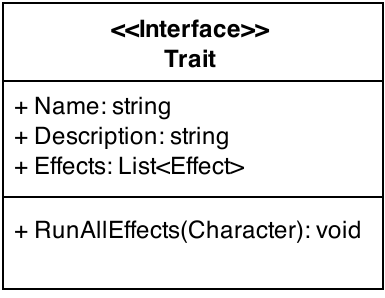
\includegraphics[width=0.5\textwidth]{figures/traits/TraitClassDiagram.png}
\caption{Trait class diagram.}
\label{traits:traitclassdiagram}
\end{figure}

\begin{figure}
\centering
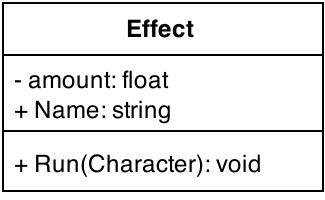
\includegraphics[width=0.5\textwidth]{figures/traits/EffectClassDiagram.png}
\caption{Effect class diagram.}
\label{traits:effectclassdiagram}
\end{figure}

% \begin{figure}
% \centering
% 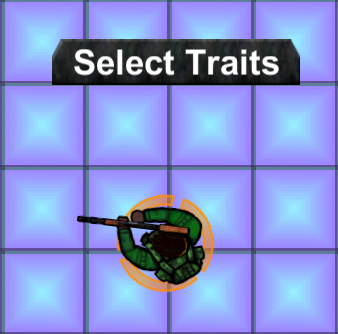
\includegraphics[width=0.5\textwidth]{figures/traits/SelectTrait.png}
% \caption{Screenshot of the \texttt{select traits} button that appears when a character levels up.}
% \label{traits:traitselection:selectbutton}
% \end{figure}

\begin{figure}
\centering
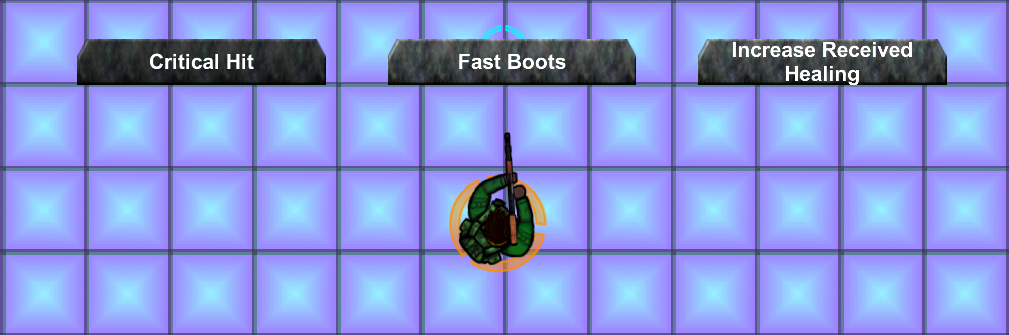
\includegraphics[scale=0.3]{figures/traits/Traits.png}
\caption{Screenshot of three traits that the player can choose from.}
\label{traits:traitselection:traits}
\end{figure}